%
%
\documentclass{article}
\usepackage{amsmath}
\usepackage{graphicx}
\usepackage{color}
\usepackage{caption}
\usepackage{amsfonts}
\usepackage[margin=3cm]{geometry}
\usepackage{tikz}
\newcommand{\cE}{\mathcal{E}}                               %

\begin{document}

\title{Small toughness solution}
\author{Tim Large, Dominic Skinner}
\maketitle
\section{Setup}
Recall we have a system goverened by the equations
\begin{equation} \left( \begin{array}{c} p(z) \\ 0 \end{array} \right) =
\int_0^{\infty} \left( \begin{array}{cc} K_{11}(x-z) & K_{12}(x-z) \\
 K_{21}(x-z) & K_{22}(x-z) \end{array} \right)
 \left( \begin{array}{c} g'(x) \\ h'(x) \end{array} \right) dx
\end{equation}
\begin{equation}
p(z) = - \int_z^{\infty} \frac{\lambda}{h(x)^2} dx
\end{equation}
where the kernel terms are given by
\[ \begin{array}{lcl}
\displaystyle K_{11}(z) = \frac{32-24z^2}{(z^2+4)^3} & &
\displaystyle K_{12}(z) = \frac{48z^2-64}{z(z^2+4)^3} \\[19pt]
\displaystyle K_{21}(z) = -\frac{(16z^3+16z^2+4)}{z(z^2+4)^3} & &
\displaystyle K_{22}(z) = -\frac{(32-24z^2)}{(z^2+4)^3} 
\end{array} \] 
with boundary conditions at infinity
\[ h''(x) \to 1, \quad g'(x) \to \frac{1}{2} \]
For a given speed parameter $\lambda$, we wish to find the material toughness
$K$, which is given by
\[ K(\lambda) = \lim_{x\to 0} 3 \sqrt{2\pi} \sqrt{x} \;h'(x) \]
We are interested in the value $\lambda = \lambda_0$ for which 
$K(\lambda_0)=0$, since this is then the propagation speed of a zero-toughness
system. We are also interested in $\lambda \approx \lambda_0$.
%
\section{Zero toughness solution}
% 
Consider setting $K=0$. We investigate only the nature of the solution near
$x=0$. We suspect, (and will verify later) that $p$ is singular near the crack
tip. Thus in equation 1, we can neglect terms that are non singular. 
\[ p(z) = -\int_0^{\infty} \frac{h'(x)}{x-z} dx \]
Also have that $p' = \lambda/h^2$. We try the ansatz $h \sim x^{\alpha}$. From
our two equations linking $h$ and $p$, this gives that
\[ p \sim x^{\alpha-1} \]
\[ p' \sim x^{-2\alpha} \]
and so $\alpha = 2/3$. We have made use of the integral
\[ \int_0^\infty \frac{x^{s-1}}{x-z}dx = -\pi \cot (\pi s)z^{s-1} \]
So starting with a solution $h_0 = A_0 x^{2/3} + o(x^{2/3})$ near the
crack tip, we get $\displaystyle p_0(x) = -\frac{2\pi A_0}{3\sqrt{3}}x^{-1/3} 
+ o(x^{-1/3})$. Putting this into the lubrication equation 
$p' h^2 = \lambda_0$, we find that 
\[ A_0 = \left( \frac{243 \lambda_0^2}{4\pi^2} \right)^{1/6} \]
{\color{red}We also can take $g_0 = Bx^{1/2}+\dots$ for $x\to0$. $B$ can only
be found numerically. (N.B. in red since this isn't an issue in \cite{GandD},
and I'm not sure where this came from or if it's even needed.)}
To recap the zero tougness solution takes the form
\begin{alignat*}{2}
h_0(x) &= A_0 x^{2/3} &+ \dots \\
p_0(x) &= -\frac{3\lambda_0}{A_0^2} x^{-1/3} &+ \dots \\
g_0(x) &= Bx^{1/2} &+ \dots 
\end{alignat*}
This holds only when $K=0$ exactly, and the above is a good approximation
for small $x$, all the way to $x=0$.
%
\section{Small toughness solution}
Now let us consider $K>0$ but take $K$ arbitrarily small. One expects for 
$K$ small, that the new solution will look much like the $K=0$ solution.
However for any small, but non-zero, value of $K$, we must have that
$h(x) \sim \frac{2K}{3\sqrt{2\pi}}x^{1/2}$ as $x\to0$. Thus the zero toughness
solution cannot be a good approximation for the entire domain. This is 
resolved by a LEFM boundary layer, following \cite{GandD}.
Outside this boundary layer, we expect behaviour close to the lubrication 
solution. So outside the boundary layer, look for a solution
\begin{align*}
g(x) &= g_0(x) + \cE(K)g_1(x)+o(\cE) \\
h(x) &= h_0(x) + \cE(K)h_1(x)+o(\cE) \\
p(x) &= p_0(x) + \cE(K)p_1(x)+o(\cE) \\
\lambda &= \lambda_0 + \cE(K)\lambda_1+o(\cE) 
\end{align*}
Where $\cE(K)$ is an unknown function of $K$ which will be determined.
We work with $K$ small enough such that $\cE(K) \ll 1$, (will be easily
verified later).
\\
\\
For definiteness, we suppose the LEFM boundary layer, with behaviour like
$h \sim x^{1/2}$ is confined to $0 \leq x \leq x_b $. If we can find some
intermediate length scale $x_b \ll x \ll 1$, then to leading order, the
asymptotics of the zero tougness solution ($h_0 \sim x^{2/3}$) will hold.
We call this region the lubrication region.
\\
\\
Recall that the expansion in $\cE$ only holds outside the LEFM boundary
layer. To find $\cE$, we will take the outer asymptotics of the LEFM boundary
layer and attempt to match that with the asypmtotics of the lubrication region. 

\begin{figure}[!ht]\centering
\caption{Matching outer asymptotics of the LEFM boundary later with the inner
asymptotics of the Lubrication region}
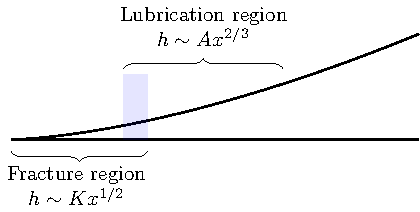
\includegraphics{Fig6.pdf}
\end{figure}

%
\section{Lubrication region}
In the lubrication region, we expect to leading order the $h = A_0x^{2/3}$
behaviour seen in the zero toughness solution. But now, looking for a term
$h = A(K) x^{2/3} + \dots$, and repeating the same calculations as before, 
we find that
\[ A(K) = \left( \frac{243 \lambda(K)^2}{4\pi^2} \right)^{1/6} =
A_0 + \frac{A_0\lambda_1}{3\lambda_0}\cE(K)+o(\cE) \]
This gives us an $x^{2/3}$ contribution to $h_1$. We posit that the remaining
contribution is, to leading order proportional to $x^s$.
\[ h_1(x) = \frac{A_0 \lambda_1}{3\lambda_0} x^{2/3} + x^s + o(x^s) \]
Any constant factor on the $x^s$ term can be absorbed into the functions 
$\cE(K)$ and $\lambda_1$. Putting this into the lubrication equation and 
taking terms linear in $\cE$ yields the equation
\[ \lambda_1 = h_0^2p'_1 + 2h_0h_1p'_0 \]
from which we obtain
\begin{align*}
p_1' &= \frac{\lambda_1}{3A_0^2}x^{-4/3} - \frac{2\lambda_0}{A_0^3}x^{s-2} \\
 &= \frac{\lambda_1}{3A_0^2}x^{-4/3} - \frac{4\pi}{9\sqrt{3}}x^{s-2} 
\end{align*}
Now we will match this with the elasticity equation. Importantly we expect 
that $p_1(x)$ is singular as $x\to 0$. Now in the elasticity integral, we have
\[p(z) = \int_0^{\infty} K_{11}(x-z)g'(x) + K_{12}(x-z)h'(x) dx \]
Now, if we estimate that in this lubrication region we have $g(x)=Bx^{1/2}$
to leading order - in other words assuming that we have nonzero $K_{II}$ -
then the pressure exerted by the horizontal dislocation $\int_0^{\infty}
K_{11}(x-z)g'(x) dx$ is non-singular as $z\to0$, and thus cannot produce
the leading order $x^{s-1}$ term we need in $p_1(x)$, so we can safely ignore
this integral.
\\
\\
Likewise, writing
\[ K_{12}(z) = - \frac{1}{z} + \frac{z^5+12z^3 +96z}{(z^2+4)^3} \]
we can treat the pressure due to the vertical dislocation as being the sum of 
a Cauchy singular integral (which has a singular response), and a 
non-singular part which produces only higher order terms in the pressure.
Accordingly, ignoring all higher order terms we obtain
\[ p_1(z) = \frac{2A_0\lambda_1}{9\lambda_0} \int_0^{\infty} 
\frac{x^{-1/3}}{x-z} dx - s\int_0^{\infty} \frac{x^{s-1}}{x-z} dx \]
However, the first term above is precisely the $x^{-4/3}$ term in the earlier 
equation for for $p_1'$; so equating the second terms we have
\begin{align*}
\frac{4\pi}{9\sqrt{3}}z^{s-1} &= s(s-1)\int_0^{\infty} \frac{x^{s-1}}{x-z} dx \\
&= s(1-s) \cot(\pi s) z^{s-1} 
\end{align*}
This is a transcendental equation for $s$ which is solved by
\[ s \approx 0.138673 \]
This then gives the form for $h_1$ in the lubrication region.
\\
\\
To recap, for $x \gg x_d$ and for $K$ very small (\& $\cE(K) \ll 1$), the 
solution is approximately the zero tougness solution
\begin{align*}
h(x) &= h_0(x) + \cE(K)h_1(x)+o(\cE) \\
p(x) &= p_0(x) + \cE(K)p_1(x)+o(\cE) \\
\lambda &= \lambda_0 + \cE(K)\lambda_1+o(\cE) 
\end{align*}
For an intermediate length scale $x_d \ll x \ll 1$ we have the asymptotics
\begin{align*}
h(x) &= (A_0x^{2/3}+\dots) + \cE(K)(\frac{A_0\lambda_1}{3\lambda_0}x^{2/3}
+x^s+\dots)+o(\cE) \\
p(x) &= (-\frac{3\lambda_0}{A_0^2}x^{-1/3}+\dots)
 + \cE(K)(\frac{2\pi A_0\lambda_1}{9\lambda_0\sqrt{3}}x^{-1/3}
+\frac{4\pi}{9\sqrt{3}(1-s)}x^{s-1}+\dots)+o(\cE) \\
\lambda &= \lambda_0 + \cE(K)\lambda_1+o(\cE) 
\end{align*}
But since we know $s$ and have $s<2/3$, so writing the $\cE$ terms to
just leading order gets that 
\begin{align*}
h(x) &= (A_0x^{2/3}+\dots) + \cE(K)(x^s+\dots)+o(\cE) \\
p(x) &= (-\frac{3\lambda_0}{A_0^2}x^{-1/3}+\dots)
 + \cE(K)(\frac{4\pi}{9\sqrt{3}(1-s)}x^{s-1}+\dots)+o(\cE) \\
\lambda &= \lambda_0 + \cE(K)\lambda_1+o(\cE) 
\end{align*}
%
\section{Fracture region}
Sufficiently close to the fracture tip, we approximate the solution as being
the solution from the \emph{semi-infinite crack} problem: as observed above, 
the integral kernels $K_{12}$ and $K_{21}$ can be split into singular and
non singular response terms. Close to the crack tip, the singular terms 
dominate, the problem decouples and we recover the familiar semi infinite
crack problem where
\[ p(z) = - \int_0^{\infty} \frac{h'(x)}{x-z} dx, \qquad
h^2p'=\lambda, \qquad h(x) \to \frac{2K}{3\sqrt{2\pi}} x^{1/2} \]
Now we make the rescalings
\[ x = \lambda^{-2}K^6 \xi, \qquad h = \lambda^{-1}K^4 \eta, \qquad
p=\lambda K^{-2} \Pi \]
which then give the dimensionless problem
\[ \Pi(\zeta) = -\int_0^{\infty}\frac{\eta'(\xi)}{\xi - \zeta} d\xi, \qquad
\eta^2 \Pi'=1, \qquad \eta(\xi) \to \frac{2}{3\sqrt{2\pi}}\xi^{1/2} \]
Now in the well known solution to this problem, we have the fracture region
in $\xi \ll 1$ and a lubrication region in $\xi \gg 1$, which is to first
approximation given by the eigensolution $\eta=\tilde{A}\xi^{2/3}$ where
$\tilde{A} = (243/4\pi^2)^{1/6}$, the same as before but without the 
$\lambda_0$ terms we have scaled out. We seek the next order in the solution
for $\xi \gg 1$, in other words, we want to expand for large $\xi$.
\[ \eta(\xi) = \tilde{A}\xi^{2/3} + C \xi^t + \dots\]
For some $0<t<2/3$. The procedure to do this is exactly as in the previous 
section, substituting this into both the lubrication and fracture problems, 
to obtain a transcendental equation for $t$, which is the same as the 
earlier one, yielding
\[t=s\approx 0.138673\]
On the other hand, the constant $C$ can only be determined numerically.
Redimensionalizing, we obtain an outer limit to the LEFM boundary solution
of the form 
\begin{align*}
h(x) &= \tilde{A} \lambda^{1/3} x^{2/3} + CK^{4-6s}\lambda^{1-2s}
x^s + \dots \\
&= h_0(x) + \cE(K) \frac{A_0 \lambda_1}{3\lambda_0} x^{2/3}
+CK^{4-6s} \lambda_0^{1-2s}x^{s} + \dots 
\end{align*}
%
\section{Matching}
We can match our two expressions for $h(x)$ together, obtaining 
\[ \cE(K) = CK^{4-6s}\lambda_0^{1-2s} \]
for a constant $C$. In particular, $4-6s \approx 3.16796$ which gives
the desired exponent. We note the length of the boundary layer scales like
$K^6$, i.e. $x_d \sim K^6$. 
\\
\\
Importantly, we get that 
\[ \lambda = \lambda_0 + C K^{4-6s} \lambda_0^{1-2s} \lambda_1 + o(K^{4-6s})\]
which will be a good approximation to $\lambda$ for $K^{4-6s} \ll 1$.
%
% References/Bibliography ////////////////////////////////////////////////////
%
%\clearpage 
\begin{thebibliography}{9}  
%
\bibitem{GandD}
Garagash, D.I., Detournay, E.,
\emph{Plane-Strain Propagation of a Fluid-Driven Fracture: Small Toughness
Solution,}
Journal of Applied Mechanics,
2005.
%
%
\end{thebibliography}
\end{document}

